So far we have discussed the spectrum of an observable, which tells us all the \emph{possible} measurement outcomes, but tells us nothing about the actual act of taking a measurement itself. This comes through axioms 3 and 5. In order to illustrate these two axioms we will repeatedly use the quantum harmonic oscillator as an example, but it is important to note the methods are not specific to this case. Any restrictions required for the methods to hold will be clearly stated. 

This lecture can be read in two ways. One could read sections 4 and 5 first (on how you prepare a given state) and then return to read sections 1-3 (on how you take measurements of this state); or one could simply read it as presented (i.e. 1-5). Both reading orders have their advantages, but we present it here in the order taught by Dr. Schuller. Also in correspondence with the lecture given, we shall also translate some of the notation into the commonly used bra-ket notation (see lecture 4), even though we do not use it in this course. All these expressions shall appear in blue. 

\subsection{Spectral Decomposition of $H$ For The Quantum Harmonic Oscillator}

Recall: We found an ON-basis of $H$-eigenvalues which we labelled $\psi_n$ obeying 
\bse 
H\psi_n = E_n\psi_n,
\ese 
with 
\bse 
E_n = \hbar\omega \bigg(n+\frac{1}{2}\bigg).
\ese 
More precisely we derived 
\bse 
\psi_0(x) = \sqrt{\frac{m\omega}{2\hbar}}\exp\bigg(-\frac{m\omega}{2\hbar}x^2\bigg),
\ese 
and 
\bse 
\psi_n(x) := A_n (a_+)^n\psi_0(x) \propto H_n\bigg(\sqrt{\frac{m\omega}{\hbar}}x\bigg)\exp\bigg(-\frac{m\omega}{2\hbar}x^2\bigg).
\ese 

The only thing we will actually use in this lecture is the fact that the $\{\psi_n\}$ is an ON-basis,
\bse 
\braket{\psi_n}{\psi_m} = \delta_{nm},
\ese 
and the fact that the spectrum is given by 
\bse 
\sigma(H) = \bigg\{ \hbar\omega\bigg(n+\frac{1}{2}\bigg)\, \Big| \, n\in\N_0\bigg\}.
\ese 

The key to understanding measurement theory in quantum mechanics is that you know the spectral decomposition of the observable(s) you want to measure. In order to obtain the spectral decomposition of $H$ we consider the projectors 
\bse 
P_n(\cdot) := \braket{\psi_n}{\cdot} \psi_n \textcolor{blue}{= \ket{\psi_n}\bra{\psi_n}.}
\ese 
Note that this operator is bounded as 
\bse 
\sup_{\varphi\in\cH}\frac{\|P_n(\varphi)\|_{\cH}}{\|\varphi\|^2_{\cH}} = \sup_{\varphi\in\cH}\frac{|\braket{\psi_n}{\varphi}|^2\|\psi_n\|^2}{\|\varphi\|^2} = \sup_{\varphi\in\cH}\frac{|\braket{\psi_n}{\varphi}|^2}{\|\varphi\|^2} < \infty.
\ese 
We can, therefore, employ the operator norm on $\cL(\cH)$ to decide convergence of the following sum with the result
\bse 
\sum_{n=0}^{\infty} P_n = \id_{\cH}.
\ese 

\bd 
For every Borel set $\Omega\in\R$, define 
\bse 
P_H(\Omega) := \sum_{\substack{n \\ E_n\in\Omega}} P_n,
\ese 
i.e. the sum over the projectors such that the energy eigenvalue corresponding to the state\footnote{Again recall $\psi_n$ are not the states themselves, $\rho_{\psi_n}$ are} corresponding to $\psi_n$ is within your Borel set. 
\ed 

\br 
From now on we shall drop the $E_n\in\Omega$ on the sum, to lighten the notation, but it is important to remember that it belongs there whenever we use $P_H$. It will prove highly instrumental to the results that follow. 
\er 

\be 
Let $\Omega=\{E_m\}$, i.e. just the set containing the single eigenvalue $E_m$. Clearly then 
\bse 
P_H(\Omega) = P_m.
\ese 
\ee 

\be 
Let $\Omega=\{E_m,E_k\}$. Then we have 
\bse 
P_H(\Omega) = P_m + P_k.
\ese 
\ee 

\bp 
The map $P_H:\sigma(\R)\to\cL(\cH)$ is a projection valued measure, and in fact corresponds to \emph{the} projection valued measure that appears in the spectral theorem for $H$. That is 
\bi{rCl}
H & = & \int_{\R}\lambda P_H(d\lambda) \\
& = & \sum_{n=0}^{\infty} E_n \cdot P_n \\
& \textcolor{blue}{=} & \textcolor{blue}{\sum_{n=0}^{\infty}\hbar\omega\bigg(n+\frac{1}{2}\bigg)\ket{\psi_n}\bra{\psi_n}}.
\ei 
\ep 

\br 
The above proposition makes sense. The Hamiltonian (the energy operator) is given by the energy eigenvalues multiplied by a projector that projects the state into a state whose energy eigenvalue was the prefactor. This is clearly just the eigenvector equation.
\er 

\br 
Note there was nothing specifically special about the fact that we were considering the Hamiltonian above. Indeed the same method holds for \emph{any} observable you wish to measure. First find an ON-basis of eigenvectors for your operator, $A$ say, and then define the PVM associated to the observable
\bse 
P_A:\sigma(\R) \to \cL(\cH)
\ese 
in the same way and then plug it into the spectral theorem. 
\er 

\subsection{Probability to Measure a Certain Value}

As stated in the opening of this lecture, the method is the same for all observables and their measurements, but we shall use the energy of the quantum harmonic oscillator as our working example. 

Recall, the spectrum of $H$ is the set of principally possible measurement outcome results. We want to show this pictorially, as it will help with understanding what's to follow. 

As we measuring anything in the real world, we need some kind of measuring device. You feed in the thing you want to take a measurement of and the meter on the device tells you the measurement value. The one slightly different, but highly important, difference to note with quantum mechanics is that the device potentially alters the thing you were measuring. We shall draw this as follows. 

\begin{center}
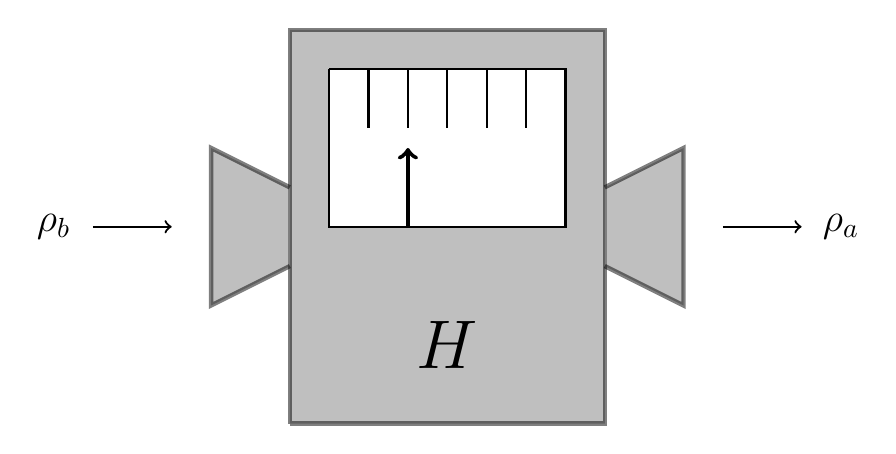
\begin{tikzpicture}
\draw[ultra thick,  fill=gray, opacity=0.5] (0,0) -- (4,0) -- (4,5) -- (0,5) -- (0,0);
\draw[ultra thick,  fill=gray, opacity=0.5] (0,2) -- (-1,1.5) -- (-1,3.5) -- (0,3);
\draw[ultra thick,  fill=gray, opacity=0.5] (4,2) -- (5,1.5) -- (5,3.5) -- (4,3);
\draw[thick, fill=white] (0.5,4.5) -- (3.5,4.5) -- (3.5,2.5) -- (0.5,2.5) -- (0.5,4.5);
\draw[thick] (1,4.5) -- (1,3.75);
\draw[thick] (1.5,4.5) -- (1.5,3.75);
\draw[thick] (2,4.5) -- (2,3.75);
\draw[thick] (2.5,4.5) -- (2.5,3.75);
\draw[thick] (3,4.5) -- (3,3.75);
\draw[ultra thick,->] (1.5,2.5) -- (1.5,3.5);
%%%%
\node at (2,1) {\Huge{$H$}};
\draw[thick, ->] (-2.5,2.5) -- (-1.5,2.5);
\draw[thick, ->] (5.5,2.5) -- (6.5,2.5);
\node at (-3,2.5) {\Large{$\rho_b$}};
\node at (7,2.5) {\Large{$\rho_a$}};
\end{tikzpicture}
\end{center}

The $H$ tells us that it is the device associated to the observable $H$, the scale markings tell us the spectrum\footnote{Here we are considering the spectrum of the harmonic oscillator, and so the notches are evenly spaced. Clearly this will not always be true. In general we have notches of varying separation as well as `blocks' for the continuous parts of the spectrum.}, the arrow tells us the \emph{actual} measurement made, $\rho_b$ is the state before the measurement and $\rho_a$ is the state after the measurement. 

\br 
Note that the pointer here will not move continuously between the notches; it moves between the values by jumping between them. In other words, it can no point at in between two notches, as this would not be part of the spectrum. 
\er 

Recall: a \emph{state} of a quantum system is a self adjoint operator that is:
\ben[label=(\roman*)]
\item Trace-class: $\Tr(\rho)=\sum_{e_n}\braket{e_n}{\rho(e_n)} <\infty$, where $\{e_n\}$ is \emph{any} ON-basis. 
\item Unit trace: $\Tr(\rho)=1$. 
\item Positive: $\forall\varphi\in\cH, \, \braket{\varphi}{\rho(\varphi)}\geq 0$.\footnote{Note that this should really be called `non-negative', however this is just how it is named.}
\een 

Also recall: Axiom 3 assorts that the probability to obtain a measurement outcome (a `pointer position') within a Borel set $\Omega$ when measuring an observable $H$ on a system in state $\rho$ is given by
\bse 
\Tr\big(P_H(\Omega)\circ \rho\big),
\ese 
where $P_H$ is the unique PVM from the spectral decomposition of $H$. In terms of our picture it asks the question `What is the probability that the pointer points within the range $\Omega$ on the scale?'
\begin{center}
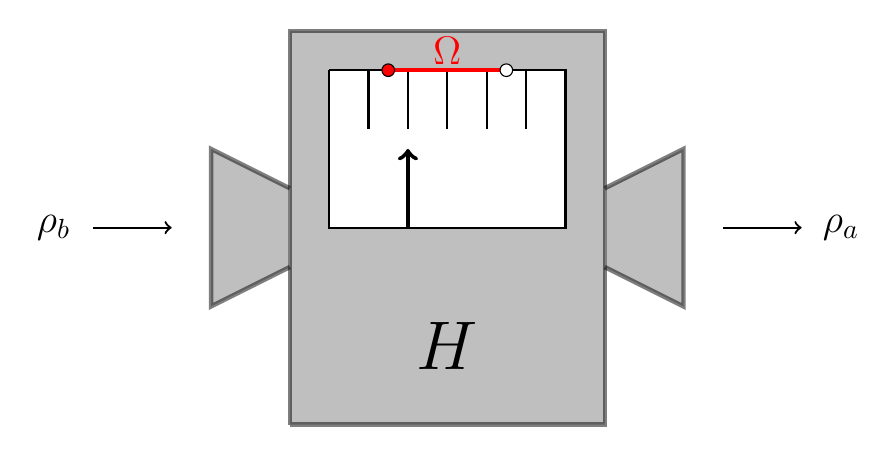
\begin{tikzpicture}
\draw[ultra thick,  fill=gray, opacity=0.5] (0,0) -- (4,0) -- (4,5) -- (0,5) -- (0,0);
\draw[ultra thick,  fill=gray, opacity=0.5] (0,2) -- (-1,1.5) -- (-1,3.5) -- (0,3);
\draw[ultra thick,  fill=gray, opacity=0.5] (4,2) -- (5,1.5) -- (5,3.5) -- (4,3);
\draw[thick, fill=white] (0.5,4.5) -- (3.5,4.5) -- (3.5,2.5) -- (0.5,2.5) -- (0.5,4.5);
\draw[thick] (1,4.5) -- (1,3.75);
\draw[thick] (1.5,4.5) -- (1.5,3.75);
\draw[thick] (2,4.5) -- (2,3.75);
\draw[thick] (2.5,4.5) -- (2.5,3.75);
\draw[thick] (3,4.5) -- (3,3.75);
\draw[ultra thick,->] (1.5,2.5) -- (1.5,3.5);
%%%%
\node at (2,1) {\Huge{$H$}};
\draw[thick, ->] (-2.5,2.5) -- (-1.5,2.5);
\draw[thick, ->] (5.5,2.5) -- (6.5,2.5);
\node at (-3,2.5) {\Large{$\rho_b$}};
\node at (7,2.5) {\Large{$\rho_a$}};
%%%%
\draw[ultra thick, red] (1.25,4.5) -- (2.75,4.5);
\draw[fill=red] (1.25,4.5) circle [radius=0.08];
\draw[fill=white] (2.75,4.5) circle [radius=0.08];
\node at (2,4.75) {\textcolor{red}{\Large{$\Omega$}}};
\end{tikzpicture}
\end{center}

\br 
We wish to emphasise this point again here. The spectrum of an observable only tells you the \emph{possible} measurements and the results of last lecture give you information on the \emph{probability} of each possible measurement. This is where the probabilistic nature enters into quantum mechanics. When a measurement is made, the result is concrete. You get exactly that result. This in tern effects the state of your system, giving a (potentially) new state. This is where the indeterminate nature of quantum mechanics enters. 

That is, prior to the measurement you can only say with what probability you get one of the possible final states, but once the measurement is made, it is exactly that one, and which final state you get depends on which measurement result you get. This is the \emph{quantum} behaviour of the system. 

As we shall see in section 5 there is another form of probability concerned with quantum mechanics, but this probability does not stem from the quantum nature of the system itself. It stems from the `ignorance' of the experimenter/the equipment in order to be able to distinguish which measurement was made. This results in what are known as \emph{mixed states}.
\er 

\subsection{Measurements of Pure States}
One can think of pure states as the most precise information one can obtain about a quantum system. Recall that any pure state can be written as 
\bse 
\rho_{\psi} = \frac{\braket{\psi}{\cdot}}{\braket{\psi}{\psi}} \textcolor{blue}{= \frac{\ket{\psi}\bra{\psi}}{\braket{\psi}{\psi}}},
\ese 
for \emph{some} $\psi\in\cH$.

\br
Again we emphasise that people often refer to $\psi$ as being the pure state itself. This might still seem forgivable, but as mentioned previously this is in fact uncountabley infinitely incorrect, as we have a complex scaling ambiguity: for any $\lambda \in \C\setminus\{0\}$,
\bse 
\rho_{\lambda\psi} = \rho_{\psi}.
\ese 
One might then say `Ok, just take the normalised $\psi$ elements,' but again this is still incorrect as multiplying by $e^{i\alpha}$ for $\alpha\in\C$ would still given the same result. One could say, then, `a state of the system is given by an element of the Hilbert space, up to arbitrary rescaling.'
\er 

Now lets employ $\Tr\big(P_H(\Omega)\circ\rho_{\varphi}\big)$ to calculate the probability to measure a certain energy of the harmonic oscillator for the state $\rho_{\varphi}$. As we are dealing with the harmonic oscillator, which has a purely discrete spectrum, we can simply make our Borel sets such that they contain only one measurement (one notch on the scale). We have then, for some ON-basis $\{e_n\}$
\bse
\Tr \big(P_H(\{E_k\})\circ\rho_{\varphi}\big) = \sum_n \braket{e_n}{\big(P_H(\{E_k\})\circ\rho_{\varphi}\big)e_n}.
\ese
Now seeing as $e_n$ need only be \emph{some} ON-basis, we are free to use our ON-eigenbasis $\{\psi_n\}$, giving\footnote{Recall that in the definition of $P_H$ the sum is taken such that the energy eigenvalue with that index is within the Borel set.} 
\bi{rCl}
\Tr \big(P_H(\{E_k\})\circ\rho_{\varphi}\big) & = & \sum_n \braket{\psi_n}{\big(P_H(\{E_k\})\circ\rho_{\varphi}\big)\psi_n} \\
& = & \sum_n \braket{\psi_n}{\sum_m\braket{\psi_m}{\rho_{\varphi}(\psi_n)}\psi_n} \\
& = & \sum_n \braket{\psi_n}{\braket{\psi_k}{\rho_{\varphi}(\psi_n)}\psi_k} \\
& = & \sum_n \braket{\psi_n}{\braket{\psi_k}{\frac{\braket{\varphi}{\psi_n}}{\braket{\varphi}{\varphi}}\varphi}\psi_k} \\
& = & \sum_n \frac{\braket{\varphi}{\psi_n}}{\braket{\varphi}{\varphi}}\braket{\psi_k}{\varphi} \braket{\psi_n}{\psi_k} \\
& = & \frac{\braket{\varphi}{\psi_n}}{\braket{\varphi}{\varphi}}\braket{\psi_n}{\varphi} \\
& = & \frac{|\braket{\varphi}{\psi_n}|^2}{\|\varphi\|^2} \\
& = & \frac{\|P_k\varphi\|^2}{\|\varphi\|^2},
\ei 
where we have used the fact that $\|\psi_n\|=1$ to get to the last line. 

We now note that although we no not require $\varphi$ to be an eigenvector of $H$, we can always express it as a linear combination of the ON-eigenbasis $\{\psi_n\}$. The following two examples shall highlight this point and demonstrate how one could almost instantly determine the probabilities of obtaining a given energy measurement given the expression for $\varphi$ corresponding to a pure state.

\be 
First imagine that $\varphi$ is an eigenvector of $H$, then we clearly have 
\bse 
\varphi = A\psi_{\ell}
\ese 
for $A\in\C$ and some \emph{fixed} $\ell$. Plugging this into the formula we obtain 
\bi{rCl}
\Tr\big(P_H(\{E_k\})\circ\rho_{\varphi}\big) & = & \frac{\|P_k(A\psi_{\ell})\|^2}{\|A\psi_{\ell}\|^2} \\
& = & \frac{\|\braket{\psi_k}{A\psi_{\ell}}\psi_k\|^2}{|A|^2\|\psi_{\ell}\|^2} \\
& = & \frac{|A\braket{\psi_k}{\psi_{\ell}}|^2\|\psi_k\|^2}{|A|^2} \\
& = & \delta_{k\ell},
\ei 
so the probability of obtaining energy measurement $E_k$ vanishes unless $\psi_{\ell}=\psi_k$, in which case we are certain to get that measurement. 
\ee 

\br 
In the above we could call $\varphi$ an energy-eigen\emph{state}. In this case the use of the word `state' is truly forgivable as all the other eigenvectors with the same eigenvalue would produce the same state (as in both cases we have the same scaling ambiguity). However, if we wish to avoid confusing ourselves, we need not say this.
\er 

\be 
\label{ex:PureStatePreparationLinearCombination}
Now let's assume $\varphi$ isn't a $H$-eigenvector, but is a linear combination, say 
\bse 
\varphi = A\psi_p + B\psi_q,
\ese 
for $A,B\in\C$ and $p\neq q$. Then we have 
\bi{rCl}
Tr\big(P_H(\{E_k\})\circ\rho_{\varphi}\big) & = & \frac{\|P_k(A\psi_p+B\psi_q)\|^2}{\|A\psi_p+B\psi_q\|^2} \\
& = & \frac{ \|\braket{\psi_k}{A\psi_p+B\psi_q}\psi_k\|^2 }{ \braket{A\psi_p+B\psi_q}{A\psi_p+B\psi_q} } \\
& = & \frac{ \|(A\delta_{kp} +B\delta_{kq})\psi_k\|^2 }{ |A|^2 + |B|^2 } \\
& = & \frac{|A\delta_{kp} +B\delta_{kq}|^2}{|A|^2 + |B|^2} \\
& = & \frac{|A|^2\delta_{kp}}{|A|^2 + |B|^2} + \frac{|B|^2\delta_{kq}}{|A|^2 + |B|^2},
\ei 
where we have used the fact that $\braket{\psi_p}{\psi_q}=0$ in the denominator and then in the last step used the fact that $\delta_{kp}\delta_{kq}=0$ as $p\neq q$. 

So we see that the coefficients $A$ and $B$ tell us the measurement probabilities. The extension to liner combinations with more elements follows trivially to give: if 
\bse 
\varphi = \sum_i c_i\psi_i \textcolor{blue}{\, = \sum_i c_i\ket{\psi_i}},
\ese 
for $c_i\in\C$ then the probability to measure energy $E_k$ is 
\bse 
Tr\big(P_H(\{E_k\})\circ\rho_{\varphi}\big) = \frac{ \sum_i |c_i|^2\delta_{ki} }{ \sum_i|c_i|^2 } = \frac{  |c_k|^2 }{ \sum_i|c_i|^2 }.
\ese 
\ee 

\subsection{Preparation of Pure States}

Axiom 5 asserts that upon measurement of $H$ the state $\rho_b$ is projected to the state $\rho_a$ given by\footnote{This is known as `wave-function collapse' in the literature. Dr. Schuller does not like using the wave analogy and so, if anything, he called this `collapse of the state'.} 
\bse 
\rho_a := \frac{P_H(\Omega)\rho_bP_H(\Omega)}{\Tr\big(P_H(\Omega)\rho_bP_H(\Omega)\big)},
\ese
\emph{if} $\Omega$ is the Borell set in which the \emph{actual}, \emph{really observed}, \emph{really having happened}, measurement (pointer reading) \emph{came} to lie --- that is it depends on the measurement result (past tense!). 

This fact, however, can be used to our advantage in order to prepare a state of our choosing. We shall consider the following two cases separately:
\ben[label=(\roman*)]
\item The observable $H$ with a discrete, non-degenerate spectrum, 
\item Allowing for degeneracy of the spectrum. 
\een 

For (i) we can prepare a pure state $\rho_{\psi_k}$ where $\psi_k$ is an eigenvalue of $H$ by the following device 

\begin{center}
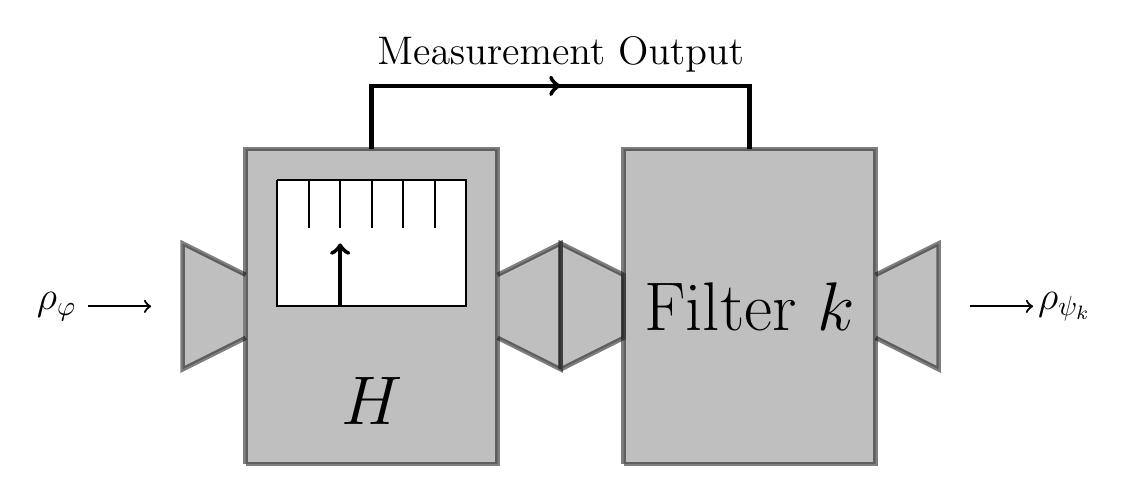
\begin{tikzpicture}[scale=0.8]
\draw[ultra thick,  fill=gray, opacity=0.5] (0,0) -- (4,0) -- (4,5) -- (0,5) -- (0,0);
\draw[ultra thick,  fill=gray, opacity=0.5] (0,2) -- (-1,1.5) -- (-1,3.5) -- (0,3);
\draw[ultra thick,  fill=gray, opacity=0.5] (4,2) -- (5,1.5) -- (5,3.5) -- (4,3);
\draw[thick, fill=white] (0.5,4.5) -- (3.5,4.5) -- (3.5,2.5) -- (0.5,2.5) -- (0.5,4.5);
\draw[thick] (1,4.5) -- (1,3.75);
\draw[thick] (1.5,4.5) -- (1.5,3.75);
\draw[thick] (2,4.5) -- (2,3.75);
\draw[thick] (2.5,4.5) -- (2.5,3.75);
\draw[thick] (3,4.5) -- (3,3.75);
\draw[ultra thick,->] (1.5,2.5) -- (1.5,3.5);
%%%%
\node at (2,1) {\Huge{$H$}};
\draw[thick, ->] (-2.5,2.5) -- (-1.5,2.5);
\node at (-3,2.5) {\Large{$\rho_{\varphi}$}};
%%%%%
\draw[ultra thick, fill=gray, opacity=0.5] (5,1.5) -- (6,2) -- (6,3) -- (5,3.5) -- (5,1.5); 
\draw[ultra thick, fill=gray, opacity=0.5] (6,0) -- (10,0) -- (10,5) -- (6,5) -- (6,0);
\draw[ultra thick, fill=gray, opacity=0.5] (10,2) -- (11,1.5) -- (11,3.5) -- (10,3);
\node at (8,2.5) {\Huge{Filter $k$}};
\draw[thick, ->] (11.5,2.5) -- (12.5,2.5);
\node at (13,2.5) {\Large{$\rho_{\psi_k}$}};
%%%%%
\draw[ultra thick] (4.5,6) -- (8,6) -- (8,5);
\draw[ultra thick,->] (2,5) -- (2,6) -- (5,6);
\node at (5,6.5) {\Large{Measurement Output}};
\end{tikzpicture}
\end{center}

We feed in a general pure state of our system into the $H$ device, which measures the energy of that pure state. It then sends this measurement output into the filter device. The state post measurement is then fed into the filter device, which is designed to only let something pass through it if the measurement was $E_k$. In this way the \emph{only} pure state that can leave is $\rho_{\psi_k}$. 

Note, although the final output is guaranteed to be $\rho_{\psi_k}$, that does not mean that the output from the $H$ device is always $\rho_{\psi_k}$ --- it could be \emph{any} of the possible output states. It is also important that $H$ is non-degenerate, otherwise the filter would let multiple different states through, all of which gave $E_k$ as their measurement output. 

For (ii) we allow for degeneracy of $H$. We overcome this by considering a \emph{maximal set of mutually commuting observables}, $\{A_1,...,A_f\}$, for which there are common eigenvectors $\psi_{a_1,...,a_f}$ with \bse 
A_i \psi_{a_1,...,a_f} = a_i \psi_{a_1,...,a_f}.
\ese 
The maximal set means that these states are uniquely determined using these operators; that is we have a subset of eigenvectors which we differentiate using this maximal set of commuting operators. The device looks like 
\begin{center}
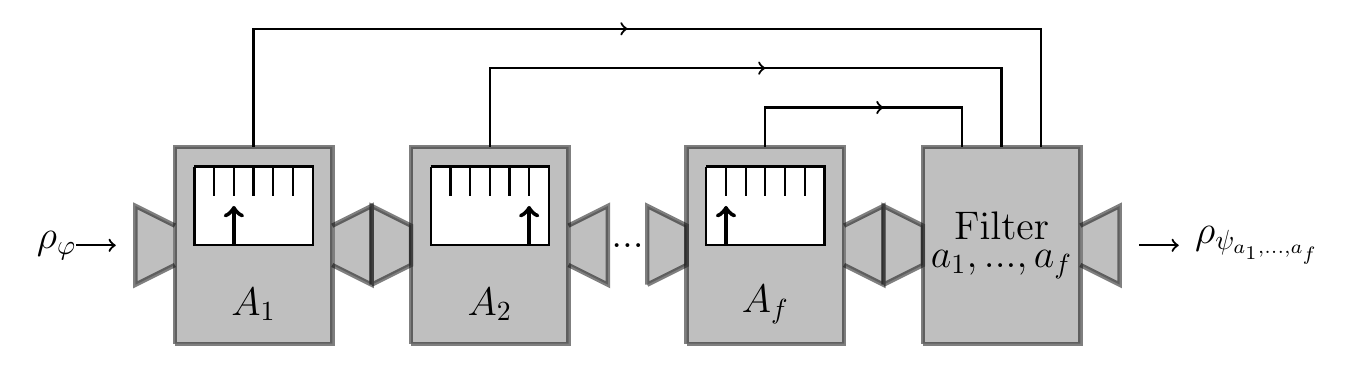
\begin{tikzpicture}[scale=0.5]
\draw[ultra thick,  fill=gray, opacity=0.5] (0,0) -- (4,0) -- (4,5) -- (0,5) -- (0,0);
\draw[ultra thick,  fill=gray, opacity=0.5] (0,2) -- (-1,1.5) -- (-1,3.5) -- (0,3);
\draw[ultra thick,  fill=gray, opacity=0.5] (4,2) -- (5,1.5) -- (5,3.5) -- (4,3);
\draw[thick, fill=white] (0.5,4.5) -- (3.5,4.5) -- (3.5,2.5) -- (0.5,2.5) -- (0.5,4.5);
\draw[thick] (1,4.5) -- (1,3.75);
\draw[thick] (1.5,4.5) -- (1.5,3.75);
\draw[thick] (2,4.5) -- (2,3.75);
\draw[thick] (2.5,4.5) -- (2.5,3.75);
\draw[thick] (3,4.5) -- (3,3.75);
\draw[ultra thick,->] (1.5,2.5) -- (1.5,3.5);
%%%%
\node at (2,1) {\Large{$A_1$}};
\draw[thick, ->] (-2.5,2.5) -- (-1.5,2.5);
\node at (-3,2.5) {\Large{$\rho_{\varphi}$}};
%%%%%
\draw[ultra thick, fill=gray, opacity=0.5] (5,1.5) -- (6,2) -- (6,3) -- (5,3.5) -- (5,1.5); 
\draw[ultra thick, fill=gray, opacity=0.5] (6,0) -- (10,0) -- (10,5) -- (6,5) -- (6,0);
\draw[ultra thick, fill=gray, opacity=0.5] (10,2) -- (11,1.5) -- (11,3.5) -- (10,3);
\draw[thick, fill=white] (6.5,4.5) -- (9.5,4.5) -- (9.5,2.5) -- (6.5,2.5) -- (6.5,4.5);
\draw[thick] (7,4.5) -- (7,3.75);
\draw[thick] (7.5,4.5) -- (7.5,3.75);
\draw[thick] (8,4.5) -- (8,3.75);
\draw[thick] (8.5,4.5) -- (8.5,3.75);
\draw[thick] (9,4.5) -- (9,3.75);
\draw[ultra thick,->] (9,2.5) -- (9,3.5);
\node at (8,1) {\Large{$A_2$}};
\node at (11.5,2.5) {\Large{...}};
%%%%%
\draw[ultra thick, fill=gray, opacity=0.5] (12,1.5) -- (13,2) -- (13,3) -- (12,3.5) -- (12,1.5); 
\draw[ultra thick, fill=gray, opacity=0.5] (13,0) -- (17,0) -- (17,5) -- (13,5) -- (13,0);
\draw[ultra thick, fill=gray, opacity=0.5] (17,2) -- (18,1.5) -- (18,3.5) -- (17,3);
\draw[thick, fill=white] (13.5,4.5) -- (16.5,4.5) -- (16.5,2.5) -- (13.5,2.5) -- (13.5,4.5);
\draw[thick] (14,4.5) -- (14,3.75);
\draw[thick] (14.5,4.5) -- (14.5,3.75);
\draw[thick] (15,4.5) -- (15,3.75);
\draw[thick] (15.5,4.5) -- (15.5,3.75);
\draw[thick] (16,4.5) -- (16,3.75);
\draw[ultra thick,->] (14,2.5) -- (14,3.5);
\node at (15,1) {\Large{$A_f$}};
%%%%
\draw[ultra thick, fill=gray, opacity=0.5] (18,1.5) -- (19,2) -- (19,3) -- (18,3.5) -- (18,1.5); 
\draw[ultra thick, fill=gray, opacity=0.5] (19,0) -- (23,0) -- (23,5) -- (19,5) -- (19,0);
\draw[ultra thick, fill=gray, opacity=0.5] (23,2) -- (24,1.5) -- (24,3.5) -- (23,3);
\node at (21,3) {\Large{Filter}};
\node at (21,2) {\Large{$a_1,...,a_f$}};
%%%%%
\draw[thick, ->] (24.5,2.5) -- (25.5,2.5);
\node at (27.5,2.5) {\Large{$\rho_{\psi_{a_1,...,a_f}}$}};
%%%%%
\draw[thick, ->] (2,5) -- (2,8) -- (11.5,8); 
\draw[thick] (11,8) -- (22,8) -- (22,5);
\draw[thick, ->] (8,5) -- (8,7) -- (15,7); 
\draw[thick] (14.5,7) -- (21,7) -- (21,5);
\draw[thick, ->] (15,5) -- (15,6) -- (18,6); 
\draw[thick] (17.5,6) -- (20,6) -- (20,5);
\end{tikzpicture}
\end{center}

\subsection{Mixed States}
Mixed states encode the `ignorance' (in the sense of lack of knowledge) on behalf of the experimenter/equipment. For example, the experimenter's inability to see exactly where the pointer is pointing, and so takes a guess at the reading. This introduces further uncertainty into which final state we obtain. It is important to note, though, that this is \emph{not} and inherently quantum mechanical property. 

The typical set up for preparing a mixed state is as follows: 

\begin{center}
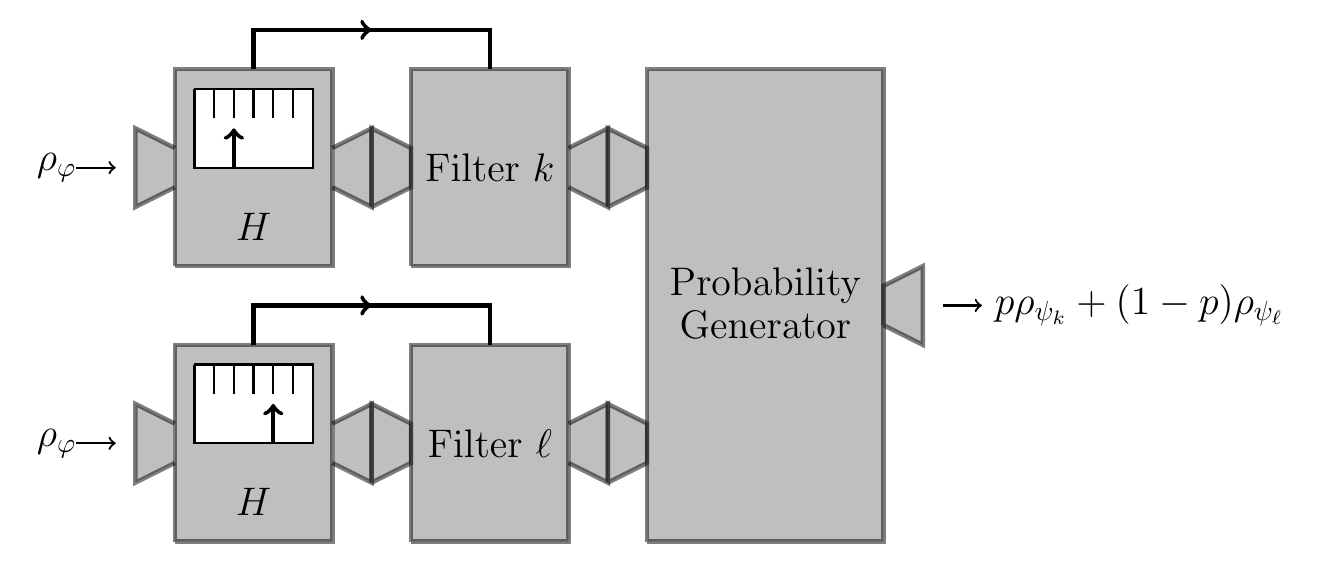
\begin{tikzpicture}[scale=0.5]
\draw[ultra thick,  fill=gray, opacity=0.5] (0,7) -- (4,7) -- (4,12) -- (0,12) -- (0,7);
\draw[ultra thick,  fill=gray, opacity=0.5] (0,9) -- (-1,8.5) -- (-1,10.5) -- (0,10);
\draw[ultra thick,  fill=gray, opacity=0.5] (4,9) -- (5,8.5) -- (5,10.5) -- (4,10);
\draw[thick, fill=white] (0.5,11.5) -- (3.5,11.5) -- (3.5,9.5) -- (0.5,9.5) -- (0.5,11.5);
\draw[thick] (1,11.5) -- (1,10.75);
\draw[thick] (1.5,11.5) -- (1.5,10.75);
\draw[thick] (2,11.5) -- (2,10.75);
\draw[thick] (2.5,11.5) -- (2.5,10.75);
\draw[thick] (3,11.5) -- (3,10.75);
\draw[ultra thick,->] (1.5,9.5) -- (1.5,10.5);
\node at (2,8) {\Large{$H$}};
\draw[thick, ->] (-2.5,9.5) -- (-1.5,9.5);
\node at (-3,9.5) {\Large{$\rho_{\varphi}$}};
\draw[ultra thick, fill=gray, opacity=0.5] (5,8.5) -- (6,9) -- (6,10) -- (5,10.5) -- (5,8.5); 
\draw[ultra thick, fill=gray, opacity=0.5] (6,7) -- (10,7) -- (10,12) -- (6,12) -- (6,7);
\draw[ultra thick, fill=gray, opacity=0.5] (10,9) -- (11,8.5) -- (11,10.5) -- (10,10);
\node at (8,9.5) {\Large{Filter $k$}};
\draw[ultra thick] (4.5,13) -- (8,13) -- (8,12);
\draw[ultra thick,->] (2,12) -- (2,13) -- (5,13);
%%%%%%%%%%%%
\draw[ultra thick,  fill=gray, opacity=0.5] (0,0) -- (4,0) -- (4,5) -- (0,5) -- (0,0);
\draw[ultra thick,  fill=gray, opacity=0.5] (0,2) -- (-1,1.5) -- (-1,3.5) -- (0,3);
\draw[ultra thick,  fill=gray, opacity=0.5] (4,2) -- (5,1.5) -- (5,3.5) -- (4,3);
\draw[thick, fill=white] (0.5,4.5) -- (3.5,4.5) -- (3.5,2.5) -- (0.5,2.5) -- (0.5,4.5);
\draw[thick] (1,4.5) -- (1,3.75);
\draw[thick] (1.5,4.5) -- (1.5,3.75);
\draw[thick] (2,4.5) -- (2,3.75);
\draw[thick] (2.5,4.5) -- (2.5,3.75);
\draw[thick] (3,4.5) -- (3,3.75);
\draw[ultra thick,->] (2.5,2.5) -- (2.5,3.5);
\node at (2,1) {\Large{$H$}};
\draw[thick, ->] (-2.5,2.5) -- (-1.5,2.5);
\node at (-3,2.5) {\Large{$\rho_{\varphi}$}};
\draw[ultra thick, fill=gray, opacity=0.5] (5,1.5) -- (6,2) -- (6,3) -- (5,3.5) -- (5,1.5); 
\draw[ultra thick, fill=gray, opacity=0.5] (6,0) -- (10,0) -- (10,5) -- (6,5) -- (6,0);
\draw[ultra thick, fill=gray, opacity=0.5] (10,2) -- (11,1.5) -- (11,3.5) -- (10,3);
\node at (8,2.5) {\Large{Filter $\ell$}};
\draw[ultra thick] (4.5,6) -- (8,6) -- (8,5);
\draw[ultra thick,->] (2,5) -- (2,6) -- (5,6);
%%%%%%%%%%
\draw[ultra thick, fill=gray, opacity=0.5] (11,1.5) -- (12,2) -- (12,3) -- (11,3.5) -- (11,1.5);
\draw[ultra thick, fill=gray, opacity=0.5] (11,8.5) -- (12,9) -- (12,10) -- (11,10.5) -- (11,8.5);
\draw[ultra thick, fill=gray, opacity=0.5] (12,0) -- (18,0) -- (18,12) -- (12,12) -- (12,0);
\draw[ultra thick, fill=gray, opacity=0.5] (18,5.5) -- (18,6.5) -- (19,7) -- (19,5) -- (18,5.5);
\node at (15,6.5) {\Large{Probability}};
\node at (15,5.5) {\Large{Generator}};
\draw[thick, ->] (19.5,6) -- (20.5,6);
\node at (24.5,6) {\Large{$p\rho_{\psi_k}+(1-p)\rho_{\psi_{\ell}}$}};
\end{tikzpicture}
\end{center}

The `probability' generator here is some method of choosing which input (left) to output (right), where there is a probability $p$ to use the top input ($\psi_k$). For example it could be a person rolling a dice that says "If I roll a `1' then I shall use the top input, otherwise I'll use the bottom one," in which case $p=1/6$. Normalisation is taken care of by requiring the other possible outcome to have probability $(1-p)$. 

\br 
It is very important to realise the the output for a mixed state is the sum of two \emph{states}; it is not the state made from the sum of two eigenvectors, as was the case with \Cref{ex:PureStatePreparationLinearCombination}. That is 
\bse 
p\rho_{\psi_k} + (1-p)\rho_{(1-p)\psi_{\ell}} \neq \rho_{p\psi_k + (1-p)\psi_{\ell}}.
\ese 
We highlight this point here as it demonstrates one of the misleading aspects of using bra-ket notation. People often talk about a pure state as one that can be written as a linear superposition of the eigenstates (as with \Cref{ex:PureStatePreparationLinearCombination}), writing 
\bse
\textcolor{blue}{\ket{\Psi} = a\ket{\psi_k} + b\ket{\psi_{\ell}} },
\ese 
for $a,b\in\C$ and $k\neq \ell$, where the normalisation condition requires $|a|^2+|b|^2=1$. But if were to think of \textcolor{blue}{$\ket{\Psi}$} as the \emph{state} then this would look like a mixed state --- it is the superposition of two pure \emph{states}. 

In order to differentiate a pure state from a mixed state they introduce the density matrices, which are the $\rho$s we've been using, and say that the density matrix of a mixed state is of the form 
\bse 
\textcolor{blue}{ \rho_{\text{mixed}} = \sum_i p_i \ket{\psi_i}\bra{\psi_i} },
\ese 
where $p_i$ is the probability of being in the corresponding state, but then going back to the start of section 17.3, we see this is just the same as what we wrote for a mixed state, without any of the potential confusion. 
\er 